\documentclass[12pt,a4paper]{article}
% Preámbulo del informe de la Etapa 3: el de la Etapa 2 sin la notación de la
% gramática. Computer Modern a 12pt, como los documentos de la cátedra, y todo en
% negro.
\usepackage[T1]{fontenc}
\usepackage[utf8]{inputenc}
\usepackage{lmodern}
\usepackage{amsmath,amssymb}
\usepackage[spanish,es-noquoting,es-noshorthands,es-tabla]{babel}
\usepackage[a4paper,margin=2.6cm,headsep=14pt]{geometry}
\usepackage{microtype}
\usepackage{booktabs}
\usepackage{longtable}
\usepackage{array}
\usepackage{xcolor}
\usepackage{fancyhdr}
\usepackage{titlesec}
\usepackage{enumitem}
\usepackage{fancyvrb}
\usepackage[hidelinks,bookmarks=true]{hyperref}

\usepackage{float}
\usepackage{graphicx}
\usepackage{pdflscape}
\DeclareUnicodeCharacter{2014}{---}
\DeclareUnicodeCharacter{2026}{\ldots}

% --- Paleta ------------------------------------------------------------------
\definecolor{tinta}{rgb}{0,0,0}

\color{tinta}

% --- Títulos ------------------------------------------------------------------
\titleformat{\section}{\Large\bfseries\color{tinta}}{\thesection}{0.7em}{}
\titleformat{\subsection}{\large\bfseries\color{tinta}}{\thesubsection}{0.7em}{}
\titleformat{\subsubsection}{\bfseries\color{tinta}}{\thesubsubsection}{0.7em}{}
\titlespacing*{\section}{0pt}{2.4ex plus 1ex minus .2ex}{1.3ex plus .2ex}

% --- Encabezado y pie ---------------------------------------------------------
\setlength{\headheight}{14pt}
\pagestyle{fancy}
\fancyhf{}
\renewcommand{\headrulewidth}{0.4pt}
\renewcommand{\headrule}{\hbox to\headwidth{\color{tinta}\leaders\hrule height \headrulewidth\hfill}}
\fancyhead[L]{\footnotesize\color{tinta}Compiladores e Intérpretes — Etapa 3}
\fancyhead[R]{\footnotesize\color{tinta}\nouppercase{\leftmark}}
\fancyfoot[C]{\footnotesize\color{tinta}\thepage}

% --- Bloques de consola --------------------------------------------------------
% \footnotesize y no \small: la línea más larga de una sesión de consola tiene
% 82 caracteres y a \small no entra en la caja de texto.
\DefineVerbatimEnvironment{consola}{Verbatim}%
  {fontsize=\footnotesize,xleftmargin=1.1em,formatcom=\color{tinta}}

\setlength{\emergencystretch}{4.5em}
\tolerance=3000

\setlist[itemize]{leftmargin=1.3em,itemsep=0.25ex,topsep=0.5ex}
\setlist[enumerate]{leftmargin=1.5em,itemsep=0.25ex,topsep=0.5ex}
\setlist[description]{leftmargin=1.3em,itemsep=0.35ex,topsep=0.6ex}
\renewcommand{\arraystretch}{1.25}

\usepackage{ragged2e}

\begin{document}

% ===========================================================================
% Portada
% ===========================================================================
\begin{titlepage}
\thispagestyle{empty}
\raggedright
\vspace*{2.2cm}

{\footnotesize\sffamily
UNIVERSIDAD NACIONAL DEL SUR\\
Departamento de Ciencias e Ingeniería de la Computación\\
Compiladores e Intérpretes --- Segundo Cuatrimestre de 2026\par}

\vspace{2.4cm}
{\rule{\textwidth}{0.6pt}}
\vspace{1.1cm}

{\Huge\bfseries Compilador de MiniJava\par}
\vspace{0.5cm}
{\LARGE\color{tinta} Etapa 3 --- Analizador Semántico I\\[0.25cm]
\large Tabla de Símbolos y Chequeo de Declaraciones\par}

\vspace{1.1cm}
{\rule{\textwidth}{0.6pt}}

\vspace{2.6cm}
{\large Agustín Paul\par}
\vspace{0.2cm}
{\normalsize L.U. 147524\par}
\vspace{0.4cm}
{Informe de entrega\par}

\vfill
{\color{tinta}\footnotesize \today\par}
\end{titlepage}

\thispagestyle{empty}
\tableofcontents
\newpage
\setcounter{page}{1}
\RaggedRight

% ===========================================================================
\section{Cómo compilar y ejecutar}
% ===========================================================================

Proyecto Maven con Java~25. Desde la carpeta \texttt{compilador/}:

\begin{consola}
$ mvn package          # compila, corre la suite y arma target/Compilador.jar
$ java -jar target/Compilador.jar programa1.java
Compilacion Exitosa

[SinErrores]
\end{consola}

El fuente es el único argumento y puede tener cualquier extensión. Sin opciones corre esta etapa,
que también se elige con \texttt{-{}-etapa=3}. Las etapas anteriores siguen disponibles:
\texttt{-{}-etapa=1} corre sólo el léxico y \texttt{-{}-etapa=2} sólo el sintáctico.

% ===========================================================================
\section{La tabla de símbolos}
% ===========================================================================

La tabla es estática y de acceso global. El sintáctico la llena con las acciones de un esquema de
traducción sobre su gramática LL(1): cada clase, interfaz, atributo, método, constructor y
parámetro se crea apenas se lo reconoce y se agrega a la entidad actual. Si el análisis sintáctico
termina sin errores, el Módulo Principal le pide a la tabla:

\begin{enumerate}
  \item \texttt{chequearDeclaraciones()}: primero, el primer nombre repetido, que se registró al
        parsear; después, cada tipo controla su herencia, la ausencia de ciclos y los tipos de sus
        miembros;
  \item \texttt{consolidar()}: cada tipo incorpora lo heredado de su ancestro, que se consolida
        antes. Los tipos genéricos se instancian o se conservan según la herencia, y ahí se
        controlan las redefiniciones y las interfaces implementadas.
\end{enumerate}

El primer error semántico termina el análisis. Las tablas se recorren en orden de declaración,
así que el error reportado es siempre el mismo.

\medskip
Los diagramas de clases (figuras~\ref{fig:tabla} a~\ref{fig:tipos}) muestran todos los campos,
constructores y métodos del código. Lo subrayado es estático y lo que está en cursiva, abstracto.
Una referencia a otra clase dibujada es una relación, rotulada con el nombre del campo y su
multiplicidad (\texttt{0..1} si puede faltar, \texttt{*} si es una colección, ninguna si es
exactamente una), y una caja sin miembros se detalla en otro diagrama. Cada entidad guarda el
token de su declaración, que es de donde salen el lexema y la línea de cada error.

\begin{figure}[H]
\centering
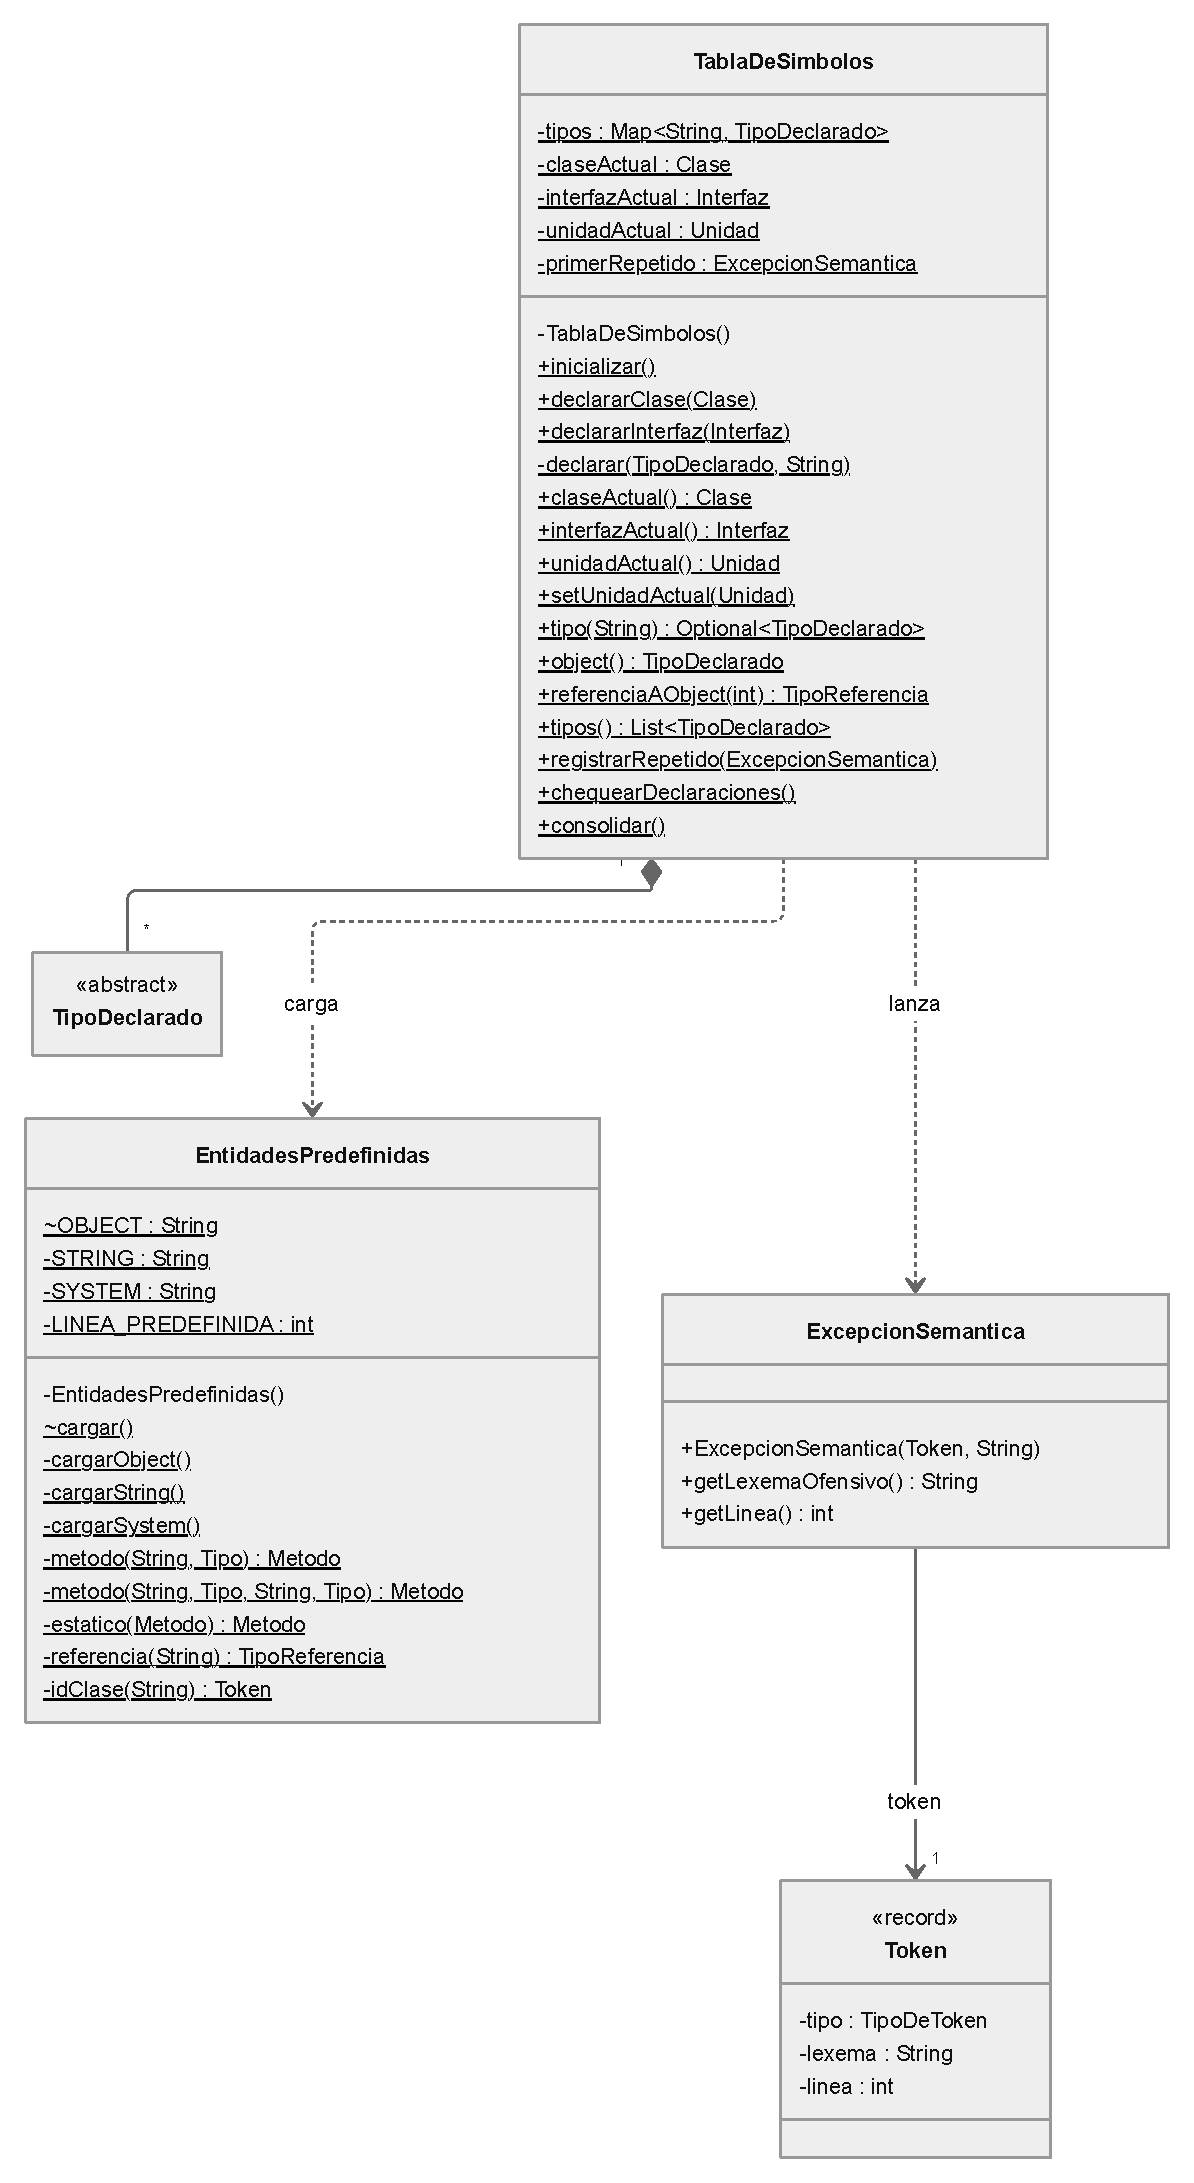
\includegraphics[width=0.82\textwidth]{generado/tabla.pdf}
\caption{La tabla de símbolos. Todos sus miembros son estáticos.}
\label{fig:tabla}
\end{figure}

\begin{landscape}
\begin{figure}[H]
\centering
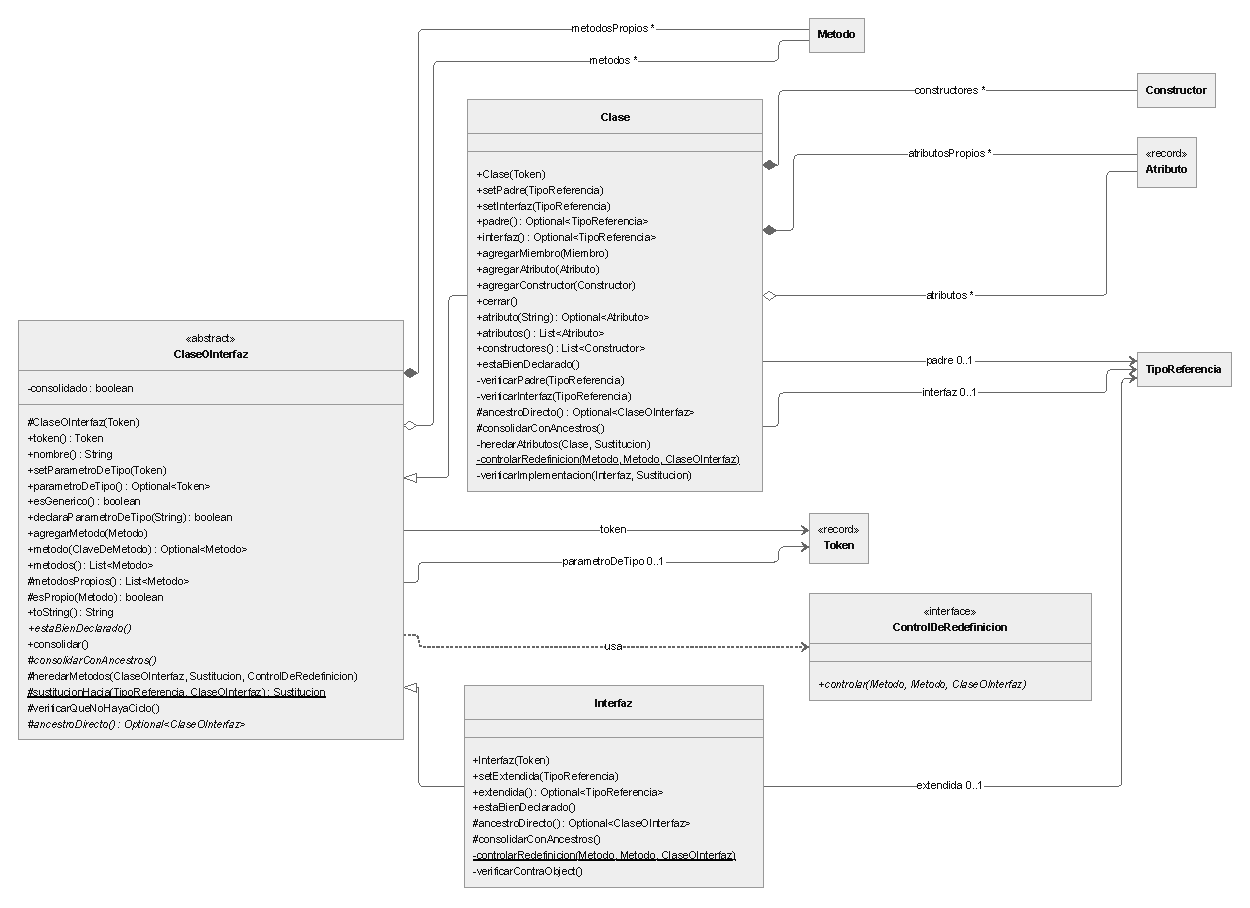
\includegraphics[width=\linewidth,height=0.86\textheight,keepaspectratio]{generado/clases-e-interfaces.pdf}
\caption{Las clases y las interfaces. \texttt{metodosPropios} y \texttt{atributosPropios} son
los declarados en el fuente; \texttt{metodos} y \texttt{atributos}, la tabla consolidada, que
suma los heredados.}
\label{fig:clases-e-interfaces}
\end{figure}
\end{landscape}

\begin{figure}[H]
\centering
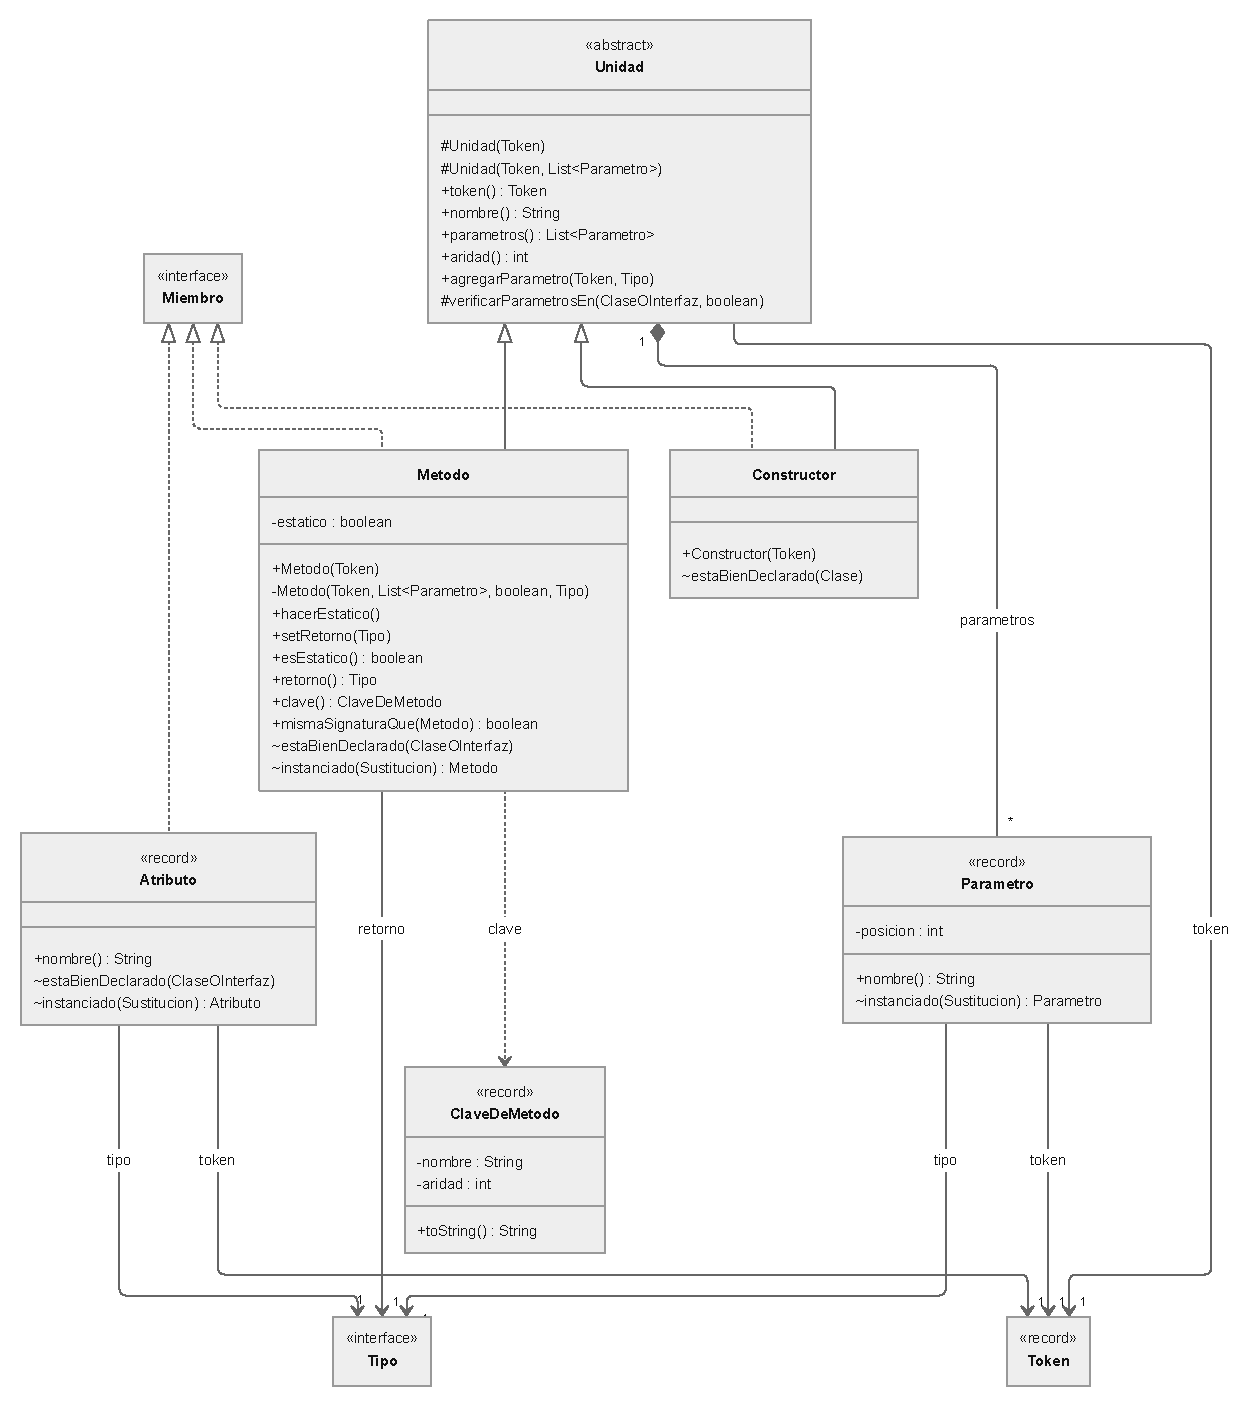
\includegraphics[width=\textwidth]{generado/miembros.pdf}
\caption{Los miembros. \texttt{Unidad} es la base de métodos y constructores.}
\label{fig:miembros}
\end{figure}

\begin{figure}[H]
\centering
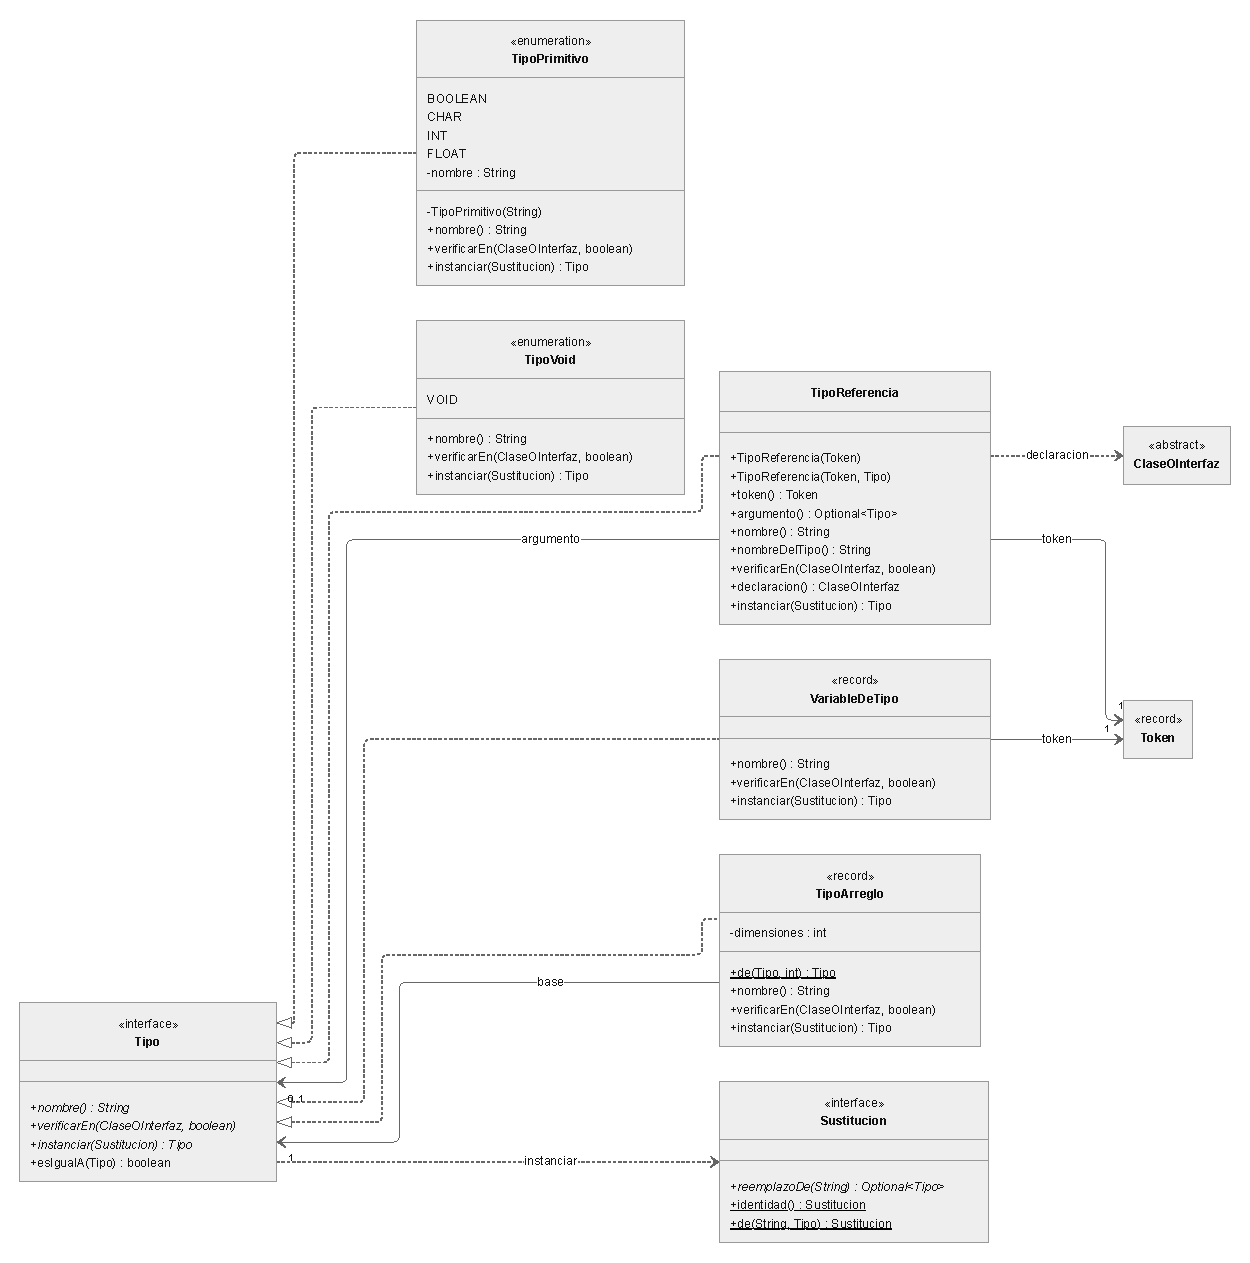
\includegraphics[width=\textwidth]{generado/tipos.pdf}
\caption{Los tipos. \texttt{Tipo} es una interfaz sellada: sólo la implementan estas cinco. Dos
tipos son iguales si se escriben igual, e \texttt{instanciar} reemplaza el parámetro de tipo de un
ancestro por el argumento de la herencia.}
\label{fig:tipos}
\end{figure}

% ===========================================================================
\section{Errores semánticos}
% ===========================================================================

Cada error se reporta como en las Pautas: \texttt{Error Semantico en linea N: ...}, un renglón en
blanco y \texttt{[Error:lexema|N]}. El token es el que fija la slide~30.

\begin{center}
\begin{tabular}{>{\raggedright\arraybackslash}p{9.6cm} >{\raggedright\arraybackslash}p{5.4cm}}
\toprule
\textbf{Error} & \textbf{Token reportado} \\
\midrule
Clase, interfaz, atributo, método (nombre y aridad), constructor (aridad) o parámetro repetido,
incluidas \texttt{Object}, \texttt{String} y \texttt{System} & la declaración posterior \\
Constructor con otro nombre que su clase & el nombre del constructor \\
Tipo no declarado, en la herencia o en un miembro & ese tipo \\
Clase que extiende una interfaz o implementa una clase; interfaz que extiende una clase & el tipo
referido \\
Argumento genérico sobre un tipo no genérico & el tipo \\
Parámetro de tipo no declarado, o usado en un método estático & el parámetro \\
Herencia circular & la primera clase declarada del ciclo \\
Atributo con el nombre de uno heredado & el atributo de la hija \\
Redefinición con otra signatura; redeclaración de un estático heredado; estático con la clave de
uno de instancia heredado; interfaz que contradice a \texttt{Object} & el método de la hija \\
Clase que no implementa un método de su interfaz & la clase \\
Implementación con otra signatura, o estática & el método, si es propio; si no, la clase \\
\bottomrule
\end{tabular}
\end{center}

% ===========================================================================
\section{Logros}
% ===========================================================================

Se intentan los logros que no requieren código:

\begin{itemize}
  \item \textbf{Entrega Anticipada Semántica I}.
  \item \textbf{Imbatibilidad Semántica I}. Los 8 casos de la cátedra dan el código exacto, y el
        corpus propio cubre cada control con al menos un caso, con error y sin él.
  \item \textbf{Kudos}.
\end{itemize}

\end{document}
